% Source for docs/static/img/replay-modes.svg. Rebuild from the repository root:
%   pdflatex -output-directory=/tmp docs/scripts/replay-modes.tex
%   pdf2svg /tmp/replay-modes.pdf docs/static/img/replay-modes.svg
%   python3 docs/scripts/prepare_rollout_svgs.py
% Keep the stage boundaries in prepare_rollout_svgs.py in sync with the row positions.
% Shared preamble for the CoMLRL training-flow diagrams. Paste it verbatim at the
% top of every diagram so each .tex stays standalone.
\documentclass[tikz,border=3pt]{standalone}
\usepackage{amsmath,amssymb,bm}
\usetikzlibrary{arrows.meta,positioning,calc,fit}

% Only these paints have dark-theme mappings (assets/_diagram-theme.scss).
\colorlet{agentA}{red!80!black}     % agent 1: policy, prompts, responses, loss
\colorlet{agentB}{blue!80!black}    % agent 2
\colorlet{learned}{orange!80!black} % learned evaluators: critic, reward model
\colorlet{update}{green!50!black}   % gradients and parameter updates
% Joint or shared quantities are black. Gray = black with fill opacity.

\tikzset{
  >={Stealth[length=3.2pt,width=3pt]},
  box/.style={draw, line width=1pt, inner sep=2.5pt, minimum height=13pt},
  policy/.style={box, rounded corners=3pt, minimum width=30pt},
  flow/.style={->, line width=.8pt},
  note/.style={font=\scriptsize, align=left},
  label/.style={anchor=west, font=\footnotesize},
}

% Replay modes: which round datasets D^(1..nu) each mode samples from, with what
% weight, and the sampled training pairs B^(nu).
% Rows are animation stages; avoid \frac and \_ (their rules animate as edges).
% Bar heights are \s pt per unit weight. lambda_decay uses lambda = 0.5, so the
% normalized weights of the K = 5 datasets (age a = 4 ... 0) are 2^(4-a)/31.
\def\s{20}
\def\colx{{126,166,206,246,286}}

% \moderow{axis y}{mode label}{w1/label1, ..., w5/label5}; weight 0 = not selected.
\newcommand{\moderow}[3]{%
  \pgfmathsetmacro{\yo}{#1}
  \node[label] at (0,\yo+5) {#2};
  \draw[black, line width=.5pt] (108,\yo) -- (304,\yo);
  \foreach \w/\t [count=\i from 0] in {#3} {
    \pgfmathsetmacro{\x}{\colx[\i]}
    \ifdim\w pt>0pt
      \draw[black, line width=.8pt, fill=black, fill opacity=.12]
        (\x-9,\yo) rectangle (\x+9,\yo+\s*\w);
      \node[note] at (\x,\yo-7) {\t};
    \else
      \fill[black, fill opacity=.1] (\x-9,\yo) rectangle (\x+9,\yo+4);
    \fi
  }
}

\begin{document}
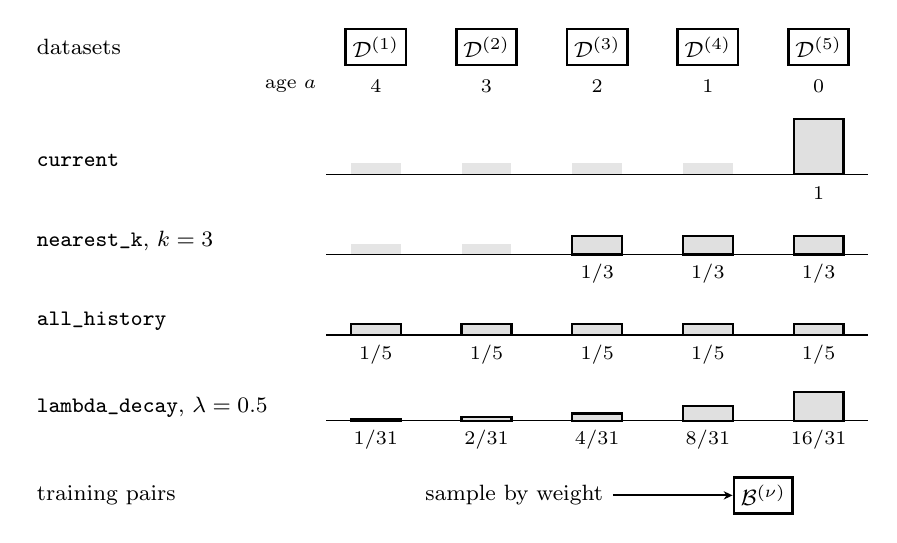
\begin{tikzpicture}[x=1pt, y=1pt, font=\footnotesize]
  % Stage 0: the round datasets, oldest left, with their ages.
  \node[label] at (0,0) {datasets};
  \node[note, anchor=east] at (108,-14) {age $a$};
  \foreach \j/\a [count=\i from 0] in {1/4, 2/3, 3/2, 4/1, 5/0} {
    \pgfmathsetmacro{\x}{\colx[\i]}
    \node[box] at (\x,0) {$\mathcal{D}^{(\j)}$};
    \node[note] at (\x,-14) {$\a$};
  }

  % Stages 1-4: selected datasets (outlined bars) and their weights.
  \moderow{-46}{\texttt{current}}{0/, 0/, 0/, 0/, 1/{$1$}}
  \moderow{-75}{\texttt{nearest\char95k}, $k=3$}
    {0/, 0/, 0.3333/{$1/3$}, 0.3333/{$1/3$}, 0.3333/{$1/3$}}
  \moderow{-104}{\texttt{all\char95history}}
    {0.2/{$1/5$}, 0.2/{$1/5$}, 0.2/{$1/5$}, 0.2/{$1/5$}, 0.2/{$1/5$}}
  \moderow{-135}{\texttt{lambda\char95decay}, $\lambda=0.5$}
    {0.0323/{$1/31$}, 0.0645/{$2/31$}, 0.1290/{$4/31$}, 0.2581/{$8/31$}, 0.5161/{$16/31$}}

  % Stage 5: pairs are sampled by dataset weight into the training pairs.
  \node[label] at (0,-162) {training pairs};
  \node (by) at (176,-162) {sample by weight};
  \node[box] (B) at (266,-162) {$\mathcal{B}^{(\nu)}$};
  \draw[flow] (by) -- (B);
\end{tikzpicture}
\end{document}
